\documentclass[doublespacing]{elsarticle}
\usepackage{amssymb}
\usepackage{amsmath}
\usepackage{bigdelim}
\usepackage{multirow}
\usepackage{hyperref}
\usepackage{graphics}
\usepackage{algorithm}
\usepackage{algorithmic}
\usepackage{subfigure}
\usepackage{booktabs}
\usepackage{url}
\usepackage{natbib}


%\usepackage{algorithmicx}
\journal{Computers in Human Behavior}

\newtheorem{definition}{Definition}


\begin{document}

\begin{frontmatter}

\begin{abstract}
 With the development of Virtual Community of Practice (VCoP), a lot
 of research was done on the mechanism and structure of virtual
 community. This paper focuses on the motivation factors of knowledge
 collaboration from system dynamics perspective. We firstly propose
 the motivation factors of users to participate knowledge
 collaboration based on community theories and  elaborate these
 factors from individual and group environment perspectives. We then
 developed a system dynamics model to demonstrate the causality of
 these factors and collaboration behavior. Next we select Wikipedia
 community as a case to test our model. The model was slightly
 adjusted to adapt to the characteristics of Wikipedia. The simulation
 result shows the model is good to reflect how these motivation
 factors affect knowledge collaboration behavior. Finally, we propose the strategy to improve the virtual community development and the future study. 

\end{abstract}

\begin{keyword}
  Virtual Community of Practice, System Dynamics, Motivation Factors, Achievement Motivation, Sense of Community, Simulation Model

\end{keyword}
\end{frontmatter}

\section{Introduction}
\label{sec:introduction}
Modern information technology enables people to communicate in a way
even not having to meet each other. Online communication gradually changes the
traditional communities to virtual communities.  A sufficient number of
people  aggregate in cyberspace and participate in  an open discussion
long enough, with sufficient emotions, setting up  their personal
relationship\cite{rheingold2000vch}. This kind of community is also
named as online community and computer mediated community. While
virtual communities may seem common to people's daily life,
researchers of knowledge management find virtual communities are great
form to better share and transfer knowledge in organizations. Members
of these communities in an organization focus their eyes on certain
topics and tasks, keep learning and practicing,  which forms virtual
communities of practice(VCoP). 

The connections between members of  VCoP are relatively weak since VCoP is
self-organized and self-maintenance. People join and quit the
communities freely at their own will. However, people keep on
attending the practice activites with great passion, contributing
their time and wisdom, under such weak
connections, usually without or just a little explicit reward from communities. Scholars and
organization managers are interested in finding what  factors drive
people to put their efforts and enthusiasm into the communities,
that is, what are their motivations.

Motivation is the dynamic factor formed by individuals collaborating the internal requirements(such as instinct, need and drive) and external cause of behavior(such as goals, reward and punishment), which can inspire and maintain the behaviors.
Sociologists and psychologists firstly studied some kinds of virtual
communities, such as online-shopping community and consumption community
modeling the internal and external impact factors and how they affect
people's behavior\cite{teo1999iae}\cite{shang2005evi}. This is because
the motivation  driving users to participate virtual community of
practice is mostly social and  psychological  motivation. Several
behavior  models
are adopted in theses studies and discuss the factors from management,
pedagogy and psychology perspectives\cite{Hsiu-FenLin04012007}\cite{bul-125-6-62719991101}\cite{Kuowiley2008}\cite{1631336620050301}\cite{Beecham2008}.

Though schoalrs propose different models of   motivation  factors to analyze communities, few of them studied
what are the interactions between these factors and how these factors
take effect together. They presume those factors are independent
implicitly in their research. The motivation of members in virtual community is
a systematic problem involving personal influence factors, group
influence factors and the relationship between different factors, and
its practical results are decided by interaction of those factors. It
is inappropriate to see these
impact factors  as independent to affect members'
behavior in VCoP. The second issue is  effect of motivation factors
may not stabilized  at a certain level in a
long duration. Due to some other factors or context change, the
motivation factors may strengthen or weaken their effect.  For these
reasons, a model can
reflect   the motivation factors interaction and
predict the change of their effect is indispensable for study of
VCoP. 

In this paper, we adopt system dynamics as our modeling
tool. The fundamentals of system dynamic modeling is its systems view
and the unique process of recognizing and  solving problems from
unity to part and from outside to inside with manifold
loops.  Recently, an increasing
number of scholars have accepted system dynamics as the tool in
virtual community research. For example, Diker  developed a
membership growth model in an open online system\cite{diker2004}. Mao etc build a system dynamics model of an online collaborative system and studied
its motivation mechanism\cite{4076734}. Wittmann and  Hattrup
adopted system dynamic to create a feedback model for information
overload\cite{wittmann_relationship_2004}. Tina presented a system dynamics model of
the evaluation system of educational techniques\cite{stavredes2001system}. Consequently, it is natural to choose system dynamics to
research the motivation factors from personal requirement and
organization environment perspectives. We developed a system dynamics
model to simulate the motivation factors, where the individual
psychological factors and the group influence psychological factors
are mainly studied. In this model, the cause and effect relationship
and the influence factors need to be verified and modified
constantly. Thanks to the computer technology and simulation software,
we identify the complicated relationship between the system factors
and the system structure. 
 
The paper is organized as follows: The next section discusses the
classification of members in VCoP. Section 3 analyzed the motivation factors
in VCoP. In section 4 we model the motivation factors based on system dynamic
to show the causality of the factors and members behavior. In section
5 we do a simulation based on data archive of Wikipedia community to verify our model.  Finally, the contributions and limitations of this study, and implications for future research are discussed.






\section{The classification of members in VCoP}
\label{sec:classification-uses}

Members in VCoP will organize themselves to work and learn together
aiming at certain topic or task, keeping  communicating and  sharing
knowledge, and achieve final output as a result. Essentially, it is a process of knowledge collaboration and knowledge-based task performance. 

Not all members in VCoP stand at the same position. Not only because of  different personalities, motivations,
behaviors and qualifications, various levels of activeness,
characteristics, ability of expression and knowledge, but more important, roles in
community interaction. Users in the same virtual community will be
differentiated and grouped spontaneously. 

Amsrtnog and Hgael classify the members into four categories from
content contribution perspective.  According to dimensions of participation and value to
the community, members are divided  into:  browser, lurker, contributor and shopper\cite{hagel1997net}. In VCoP, individuals are attracted
by topics they are interested in before they devote themselves to the
related community. Inclined to join the community as they are, whether
they can be converted from simple browsers to community users who will
enter the community repeatedly, interact with others and contribute
knowledge, depends on the amount of their interest and
satisfaction. Adler and Christopher presented the four types of
users as passive member, positive member, inductor and
manager\cite{Christopher1998}. After a long time of observation of
game-programming MUD virtual community, Bartle classified the users as killers, achievers, socializes and explorers according to their motivation and related behaviors\cite{mud}. Kozinest, when studying the consumer virtual communities, divided the members as tourist, mingler, devotee and insiders based on the relationship between users and consuming activities and relationship between users and virtual communities\cite{Kozinets1999252}. According to Kozinest, the final identification depends on two related factors: the degree of the relationship between individuals and certain consuming behaviors, and the social relation between individuals and other members in the community. 


Those researches provides dimensions to classify members: activities,
contributions and relationships. Members are differentiated from what
they did in communities, what they provide to communities and how they connected to
each others.

The main practices in VCoP  are
knowledge collaboration.  Participants actively dive into
 clearly defined  practices, leading to definite and explicit
 output. The output
 usually are knowledge product.  Knowledge transfer and sharing occurred 
 in the collaboration process. These activities classify members in
 VCoP into two groups: knowledge providers and knowledge
 receivers. Knolwedge providers are those  who are knowledgeable and willing to
  provide their knowledge by presentation, works and behaviors. They
  either provide the related knowledge to solve the problems presented
  by other members, or post messages in the community to introduce
  their experience and techniques. On the other hand, knowledge receivers learn
  and understand knowledge by imitation, listening and
  reading.  

Maintaining a VCoP needs a lot of efforts including not only  knowledge
provision, but organize practices, propose and select subjects of
practices, prepare document and some other management work. All of
them are seen as contribution to the communities. These
works are often  done by leaders and managers of communities.

  

In VCoP,  the relationships between members
in VCoP are primarily "mentorship". The relations are usually one-direction between those "pure" knowledge providers and receivers. To
senior members in communities, mentorship are usually two-directions,
that is,  the roles change rapidly in the collaboration process,
which leads to higher level knowledge collaboration and cooperation.
   
Based on above discussion,
we classify the members in VCoP into two categories because of the
relatively pure and simple relationship:   Experienced members and  ordinary members.

\begin{itemize}
\item   Experienced members: Experienced members are opinion leaders with highest influence. They are most familiar with the related information and knowledge, also they are willing to interact with others and provide their assistance. Generally, they are the most passionate and active members in the community, not only contributing their original product but also organizing or participating in discussions or activities as much as possible. 

\item  Ordinary members: ordinary members are members who just
participate in the community and those browsers. The former, lack of
strong social relationship with others, usually browse casually and
contribute little to the community. Moreover, they are inclined to
dive in the community, and obtain the knowledge they need without much
contribution. The browsers mean tourists who browse and learn in the
community with little contribution to it. 
\end{itemize}

We see the  experienced members roughly equal to insider and
devotee. Most of the contribution to VCoP are from them. They
lead the practices in VCoP, participating in the activities or
discussions initiated by others, and then offering his advice and
methods. Also they play mediating roles between community members and community operators, in charge of everyday concerns.
 The ordinary members equal to browser and lurker. They are followers
 to experienced members and make little contribution due to lack of
 knowledge and unfamiliarity to community culture. Acquiring knowledge
 from others passively by taking part in practices are their normal
 activities. Since these two categories have different activities, and
 relative status in VCoP, their motivation factors are different too.



\section{Motivation factors analysis of knowledge collaboration in virtual community of practice}
\label{sec:motiv-fact-analys}


 Dholakia et al. \cite{dholakia2004241}divides the users' motivation
 to participation as two types: One is the motivation on the
 individual level, including achieving goals, maintaining social
 relationship, social reinforcement and entertainment; The other is
 the motivation on the group level, including internalization and
 recognition. It refers to the social influence factors affecting the
 members' participation in the virtual community. Therefore, we study the motivation factors affecting the members' participation in the virtual community from two aspects: the individual level and group level.  

\subsection{Individual level motivation factors}
\label{sec:individual-level}

Motivation can be basically categorized into intrinsic motivation and
extrinsic motivation considering their "origin". Intrinsic motivation
inherently  stems from individuals themselves, referring to doing something because it is interesting or enjoyable. Extrinsic motivation refers to doing something
because it leads to a separable outcome.  It focuses on the efficacy
of the activities, which are regarded as a tool to achieve the goal. Piles of research have
shown that the different quality of experience and performance can be achieved
when one is behaving for intrinsic versus extrinsic
reasons\cite{Ryan200054}.  Extrinsic motivation is generated by
objective factors other than individuals themselves. It focuses on the
efficacy of the activities, which are regarded as a tool to achieve
the goal. Besides, extrinsic motivation can be observed and felt and
it is acquired by the exchange of material, energy and
information. Intrinsic motivation stems from individuals themselves
and involving in the activities without any effect of external
force. It focuses on the process of activities instead of the
efficacy, including sense of responsibility, sense of achievement and
need for achievement, and so on. 

Intrinsic and extrinsic motivation have different effect to motivate people\cite{deci1985ima}. A large quantity of empirical studies have proved the important role
of extrinsic motivation as incentives to promote effort and
performance\cite{gibbons1998io}\cite{388530120001201}. While
psychologists concern the great effect of intrinsic
motivation\cite{bul-125-6-62719991101}\cite{wilson1981aas}. It is hard
to determine what kind of  factors
take the priority. Furthermore, some of virtual communities solely 
developed by the enthusiasm of users instead of extrinsic
rewards. Therefore, we regard intrinsic motivation is as important as extrinsic
motivation. Intrinsic motivation is generated from the altruism of
individuals and the satisfaction of the psychological needs, or from
the pursuit of some certain moral principles. Intrinsic motivation is
mostly the satisfaction of some certain psychological
needs\cite{josh_lerner_simple_2002}. In this paper we propose 
the extrinsic and intrinsic 
motivation factors on the individual level  as the
follows: 


\subsubsection{ Information value}

Information value contains acquiring
  information, learning to handle affairs, providing information and
  contributing all the knowledge to a pool of
  information\cite{flanagin2001internet}. People attend the
  communities to get and share knowledge\cite{dholakia2004241}. Information value is not only the result of
  virtual community of practice but also the primary factor of members
  to participate in the community. It is usually the direct benefit
  from communities, especially for ordinary members.   

  \subsubsection{Instrumental value}
\label{sec:instrumental-value}
  
Participating practices in VCoP will bring certain particular value or
be conducive to a final value\cite{Roennow-Rasmussen2002}. 
Participants will complete a certain task through
online interaction, such as solving a problem, providing an original
view, affecting others, and evaluating a decision. These tasks are all
instrumental, which is often defined as the easiness to achieve the
specific goals. Flnagani and Metgze argue that instrumental
value(instrumental need) means view generation, negotiation, problem
solution, finding others for assistance and decision
making\cite{flanagin2001internet}. Instrumental value are seen as
another important extrinsic earnings as information value\cite{dholakia2004241}.

\subsubsection{Extrinsic rewards}
\label{sec:extrinsic-rewards}


   Generally, in virtual communities the rewards are
  not  in material. However, larger personal spaces and more
  privilege for functions have become the extrinsic motivation factors
  for users to participate in the community practice.  More
  importantly,  praise from other members and
honorary recognition will bring great satisfaction which compensate
their effort to the communities, in turn motivate them keep
attending the practices\cite{Zhugea}.

\subsubsection{Reciprocity}
\label{sec:reciprocity}

Everyone is limited to his abilities. Acquiring knowledge form others
is becoming more and more frequent because of the complexity of tasks
or problems. People sharing their knowledge have the expectation that
they will gain knowledge payback.  Usually, reciprocity is not realized simultaneously, but the
efficiency could be improved by interaction and mutual assistance.

\subsubsection{Need for achievement}
\label{sec:need-achievement}


 Need for achievement  describes the individuals' requirements for
success and best performance.  People  strive for success when they are performing a
task. The inner drive force of people to do those tasks perceived
are important and valuable\cite{mitzel1982encyclopedia}. It is defined as achievement
motivation.  Achievement
motivation are also seen as the competition for excellence or the hope for realizing
one's goals\cite{clark1994emc}.  
Elliot also argued  the achievement motivation is the
competition-based emotion, cognition, activation and orientation of
behaviors\cite{elliot1999aaa}.  People
with strong need for achievement aspire to do things in a perfect way,
improve working efficiency and become more successful\cite{mcclelland1976am}. They are
concerned with the joy in overcoming difficulties, solving problems
and the sense of achievement after success, but material award is not
their concern. The sense of achievement is closely related with the
development of economics, culture, society and government, as well as the
social moralities. The  individuals' sense of achievement  is
satisfied in the practice, which inversely encourages the individuals
to participate in the virtual community. 

\subsubsection{ Need for power}
\label{sec:need-power}

It is the requirement of affecting or controlling
others without being controlled. Also, it refers to the drive to
control and influence others. The extent of aspire for power
varies. Those who are endowed with a strong aspire for power are
interested in controlling, ordering, and claiming for
power. Correspondingly, they are typically argumentative, talkative,
straight, and clear-minded; they are born instructors and
lecturers. They pursue excellence and competitive environment not for
the sense of achievement as those with strong need for achievement,
but for acquiring power and status or maintaining the present
power. One kind of participants, called community leaders in virtual
community, whose advice can influence other members to a great degree,
will make lectures and instruct others when there is a debate, and
later they will obtain higher status and power in the community. 

\subsubsection{ Need for affiliation}
\label{sec:need-affiliation}

It is the need to establish intimate social
relationship, and a desire to seek for being loved and
accepted. People with strong need for affiliation are fond of
associating with others, which brings joy to them. Sensitive to
interpersonal relationship, they prefer cooperative to competitive
working atmosphere, and need more communication and mutual
understanding. Sometimes, this kind of need is presented as the fear
to lose intimate relationships and the withdraw in front of
interpersonal conflict. In virtual communities, the need for
affiliation is important to keep social association and harmonious
interpersonal relationships.

\subsubsection{Self-efficacy}
\label{sec:self-efficacy}

Self-efficacy is a significant intrinsic motivation factor which
helps to initiate knowledge collaboration between community
members.  Among personal
achievements, self-efficacy is a vital category which is defined as
individuals' perception or belief of their ability to control the
life\cite{bundura1977slt}. The behavior of individuals not only depends
on their willpower but also on their self-assurance of the effective
use of power, which can be realized by self-efficacy. As a latent
important factor affecting knowledge collaboration, self-efficacy is
the belief of the organization and execution ability needed for the
expected condition. In the context of achievement, self-efficacy is an intuitive
or personal judgment made by an individual on whether he is competent
for the task before undertaking it. It is both self-perception of
competence and an emotional private experience. Lower self-efficacy,
that is, if the members  believe their knowledge has no
or little effect to the
communities, the motivation to contribute knowledge will be
weakened\cite{1631337020050301}\cite{Hsu2007}. 

\subsection{Group level}
\label{sec:group-level}

Virtual community is a social group formed by the aggregation of
online users. Since the sociality is a typical feature of virtual
community, social factors are crucial in motivating members to
participate in virtual community. Individual motivation factors,
whether intrinsic or extrinsic, are perception of oneself, having
little relation to others' reflection. While group level motivation
factors are highly connected with the group activities. Whether these
factor can take effect  greatly depend on other peoples' response.  The sense of community, which is a
combination of the sense of belonging, sense of identity, emotional
connection and the feeling of stability, reflects the need for others
and the interaction with others of each individual. Furthermore, there
will be active impact of the sense of community. Mcmillan and Charvis
present the most influential and typical definition of the sense of
community, that is, the sense of belonging, the perception of
important relationships and community significance, and the common
belief that the group is obliged to meet the members鈥?needs\cite{mcmillan1986scd}. Although there is no face-to-face
interaction and regional association in the computer-based virtual
community, the sense of community will be derived from it. The
anonymity (the real identity will not be exposed) and selectivity
(people can enter or leave the community at any time) enables people
to explore themselves and build identity more freely, thus brings a
more interactive and open society. Therefore, virtual communities
could meet the needs of sense of community that much more than real
communities provides. In this study, we define community identity, community attachment, community cohesion, and community satisfaction as four fundamentals of the sense of community in virtual communities.      

\subsubsection{Community identity}
\label{sec:community-identiy}

Community identity involves the semiotic significance and social value
for people. It is the process and extent of the community becoming the
self-identity of individuals, similar to the sense of
membership. Sense of identity is the extent individuals feel
themselves as part of the group and studied from cognitive, afflictive
and evaluative aspects in existing
researches\cite{dholakia2004241}. From the view of cognition, identity
is a process of classification, which means the extent of
individuals鈥?recognition of themselves as a member in the virtual
community (similar with the members and different from non-members) ; From the view of affiliation, identity means the emotional state of belonging to a virtual community; Evaluation is what users evaluate themselves in the virtual community. The extent of the sense of identity varies with different individuals or groups\cite{warren1972ca}.     

\subsubsection{Community attachment}
\label{sec:community-attachment}

Community attachment is the emotional engagement in the community. The
individuals participate in virtual communities to escape from
loneliness and communicate with people of the same thoughts, obtain
friendship and social support and  form mutual emotional relationship.
Being isolated from the group affect their motivation negatively. The members will tend to participate owning to their sense of the membership. Postmes argues that the attractiveness of virtual communities comes from the sense of cluster, which is a positive experience of members gathering  to communicate with each other in the virtual community\cite{t_postmes_formation_2000}.     

\subsubsection{Community cohesion}
\label{sec:community-cohesion}

Community cohesion emphasizes on the group interaction and the
unity between individual goals and group goals. The group may influence
the expectations of individual and  integrate and realize their
needs. when they share the same sense of
worth with others, internalization of community cohesion occurs.
 The
internalization means making decisions based on the overlap between
one鈥檚 sense of worth and others' sense. Eagly and Chaiken indicate that the
sense of worth covers a large quantity of concepts, such as belief,
attitude and other moral belief\cite{eagly1993pa}. People tend to work
with those have similar opinions and experience. Also knowledge
collaboration  easily occur among members who have similar background.  Owning to the casualness of selection,
community members could select the virtual group that share
the same sense of worth with themselves at their will. Bagozzi and Dholakia
view internalization as an important influential factor of community
members\cite{richard_p._bagozzi_intentional_2002}. Internalization develops in the information exchange among
community members and keep growing when the information means a lot to
the participants. 

\subsubsection{Community satisfaction}
\label{sec:comm-satisf}

Community satisfaction has often been linked to the level of satisfaction with a
community infrastructure,  opportunities and social support networks\cite{filkins2000predicting}. It is an emotional state of community
evaluation, referring to the
subjective evaluation of the objective condition in the community and
can be differed to the real condition. Three aspects are proposed to
measure satisfaction to a community: satisfying users' social needs, adequacy of the information content for
user needs, and user satisfaction with the VC\cite{lin2006determinants}. Higher satisfaction brings
higher stickiness to the communities, which in turn leads to higher
loyalty\cite{linhsiufen2008}. Oliver also suggested that satisfaction
feeds back into the system and influences subsequent interaction and
behavior\cite{oliver1980cognitive}. Thus we adopt community
satisfaction as an important motivation factor.

The motivation factors of  individual level and group level are
presented in table \ref{tab:individual-level}.

\begin{table}[htpb]

  \centering
   \caption{the classification of motivation factors for the virtual
    community members to participate in knowledge collaboration}
\begin{tabular}{ccc}
    \toprule
    \multicolumn{ 1}{c|}{Individual level} & \multicolumn{ 1}{|c|}{extrinsic motivation} & Information value \\
    \multicolumn{ 1}{c|}{} & \multicolumn{ 1}{|c|}{} & Instrumental value \\
    \multicolumn{ 1}{c|}{} & \multicolumn{ 1}{|c|}{} & Extrinsic rewards \\
    \multicolumn{ 1}{c|}{} & \multicolumn{ 1}{|c|}{} & Reciprocity \\\cline{2-3}
    \multicolumn{ 1}{c|}{} & \multicolumn{ 1}{|c|}{Intrinsic motivation} & Need for achievement \\
    \multicolumn{ 1}{c|}{} & \multicolumn{ 1}{|c|}{} & Need for power \\
    \multicolumn{ 1}{c|}{} & \multicolumn{ 1}{|c|}{} & Need for affiliation \\
    \multicolumn{ 1}{c|}{} & \multicolumn{ 1}{|c|}{} & Self-efficacy \\\hline
    \multicolumn{ 1}{c|}{Group level} & \multicolumn{ 2}{|c}{Community identity} \\
    \multicolumn{ 1}{c|}{} & \multicolumn{ 2}{|c}{Community attachment} \\
    \multicolumn{ 1}{c|}{} & \multicolumn{ 2}{|c}{Community cohesion} \\
    \multicolumn{ 1}{c|}{} & \multicolumn{ 2}{|c}{Community satisfaction} \\
    \bottomrule
    \end{tabular}
  \label{tab:individual-level}
\end{table}

 

\section{The causality of motivation factors and human behavior}
\label{sec:modeling-process}

There are  mutual effect, either supportive or restrictive, among the
intrinsic and extrinsic motivation factors on individual level, and the same
relationships exist among factors of  individual level and group
level. 

Piles of studies have investigated crowding effect of intrinsic and
extrinsic motivation. Most of them focus eyes on crowding-out
effect. Intrinsic motivation can be impaired or replaced by extrinsic
motivation\cite{bul-125-6-62719991101}\cite{deci2000agp}\cite{kasser2002hpm}. People
tend to repeat simple work but reluctant to do innovative work\cite{amabile1998kc}\cite{schwartz1993cad},
actually decrease the performance form long
run\cite{Kruglanski1978}. On the other hand, some scholars believe proper
extrinsic motivation can promote people's autonomy and enhance
intrinsic motivation as affirmation to  performance of individual\cite{eisenberger1999eri}\cite{eisenberger1999dpp}\cite{eisenberger1997csr}.          

 Group  level motivation take direct effect to members' behavior in
 VCoP,  also interact with individual
level motivation. David Mcmillan and David
Chaves summarize  the common experience and interaction embodies
important psychological rules. Firstly, the more people interact with each
other, the more intimate they will be; The more active the experience
and relationship is, the more close the relations will
be. Secondly, achievements promote cohesion, but uncertain
interactions and the non-completion of community tasks will prevent
the community cohesion. Thirdly, spiritual connections  also
influence attitude to communities greatly. 
\cite{mcmillan1986scd}. Dholakia propose the object value of individuals will
strengthen their sense of identity, which brings the common sense of
members resulting in the community
cohesion\cite{dholakia2004241}. Bagozzi etc argue the sense of identity will increase the
individuals' desire, which is reflected as various psychological
requirements. Moreover, active
emotion expectations will increase the individuals' psychological
desire\cite{richard_p._bagozzi_intentional_2002}.  Based on the above analysis, we conclude the basic
cause-and-effect relationship between motivation factors in virtual
communities of practice shown as fig. \ref{fig:cause-and-effect}.
\begin{figure}[htpb]
  \centering

  \scalebox{0.8}{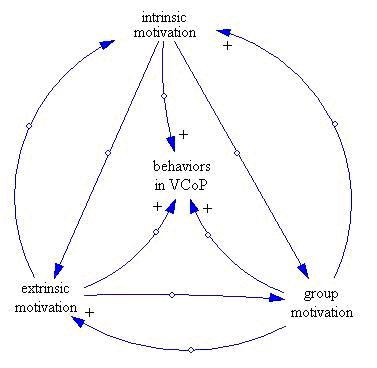
\includegraphics{02}}
  \caption{The basic causality of
    motivation factors and human behavior in VCoP}
  \label{fig:cause-and-effect}
\end{figure}

\subsection{The motivation factors model of experienced members}
\label{sec:motiv-fact-model}

 Experienced members are main force to
 participate in the knowledge collaboration and discussion. In this model the behavior
 dimension includes two horizontal variables: collaboration and
 communication. 

   On the individual level, experienced members will focus on the
   instrumental value of the community and the extrinsic rewards will
   have effect on some of them. Reciprocity is also meaningful for the
   experienced members. Because 
   solving problems, instead of acquiring information are the main
   reason of collaboration, the information
   value is relatively small to experienced member . In general,
   experienced members have stronger need for achievement, and some of
   them have stronger need for power or need for affiliation. They
   would like to undertake the responsibility and complete the task
   with some achievement, so their self-efficacy is higher and has
   positive impact on themselves. On the group level, experienced
   members have become regular members in the community, with their
   sense of identity, belonging, cohesion, and satisfaction at a
   higher level. Those psychological factors will correspondingly
   prompt them to participate in the collaboration more
   frequently. Consequently, the motivation factor dimension includes
   11 horizontal variables: instrumental value, extrinsic rewards,
   reciprocity, need for achievement, need for power, need for
   affiliation, self-efficacy, community identity, community
   attachment, community cohesion, and community satisfaction. The
   motivation factor model of experienced members is shown as fig. \ref{fig:senior_member}.
\begin{figure}[htpb]
  \centering

  \scalebox{0.8}{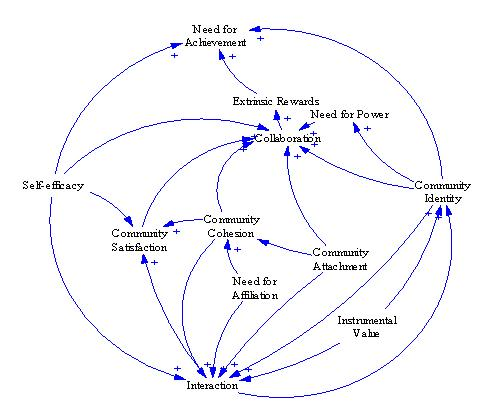
\includegraphics{03}}
  \caption{Model of motivation factors for experienced
    members in VCoP}
  \label{fig:senior_member}
\end{figure}

\subsection{The motivation factors model of common members}
\label{sec:motiv-fact-model-1}

For common members, their behavior in virtual communities are mainly
guided and taught by senior members. They take part in practices,
browsing and learning, to amplify knowledge and skills. Browsing is the only horizontal variable in the behavior dimension in this motivation factor model of common members. 


On the individual level, common members often lay great emphasis on
the information value and instrumental value of the community in
practice. Without undertaking important tasks, there is rarely any extrinsic
rewards and reciprocity between members. Although there are only a few
common members who contribute  to the community, there are still some
latent need for achievement and need for affiliation. And there is
little need for power among them. Because their behavior is mainly
browsing that is seldom affected by self-efficacy, we do not involve self-efficacy in this model. On the group
level, the common members' sense of identity, belonging, cohesion and
satisfaction is weaker compared to the experienced members, but these
psychological factors will spur them to participate in the
collaboration. Therefore, the motivation dimension includes 8
horizontal variables: information value, instrumental value, need for
achievement, need for affiliation, community identity, community
attachment, community cohesion, and community satisfaction. The
motivation factor model of common members is shown as fig. \ref{fig:common-member}.  
\begin{figure}[htpb]
  \centering
 
  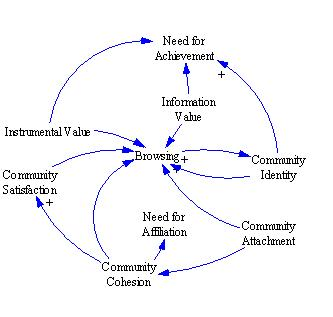
\includegraphics{04}
  \caption{Model of motivation factors for common
    members in VCoP}
 \label{fig:common-member}
\end{figure}

\section{Simulation research }
\label{sec:simulation-research-}

 We  verify our model through system simulation in this section. The model
 is moderated according to
    Wikipedia characteristics, and  a comparative
    analysis is made between the simulation results and the real
    data. 

\subsection{The background of simulation research: Wikipedia}
\label{sec:backgr-simul-rese}
Nowadays Wikipedia has been the world largest online
encyclopedia. Millions of people work together to add content to it
even without knowing each other. Wikipedia provides a few easily
handled tools allowing people edit the content collaboratively. People
of different background join the community to complete comprehensive
and accurate articles. The huge amount of  members and collaboration
activities make Wikipedia  a good example of VCoP
for our study. 
 


Wikipedia foundation download and archive the comprehensive data
periodically.  They provide three  kinds of  data archives to download
for different usage . In this paper, we select the meta history version including  meta
data of pages with complete page edit history.\footnote{http://download.wikimedia.org/enwiki/20090731/enwiki-20090731-stub-meta-history.xml.gz}.
   

A system is a functional aggregation with distinct and interactive
parts connected to each other. We  first define the boundary of
system and make primary feedback analysis before modelling. In
Wikipedia community, collaboration activities are mainly edit and
talk. Users edit page entries together through online platform,
and discuss when contents of the entry are unclear or need to make a choice . This
study describes virtual community of practice in two perspectives: a)
the result of users' practice; b) the psychological factors prompting
the generation of practice results, including factors on the
individual level and group level.

\subsection{The elements in the simulation model
}
\label{sec:defin-fact-wiki}

Due to the limitation of the data archive which can not fully reflect
the intention, we simplify our model and some of motivation factors
are not included. We omit extrinsic motivation for extrinsic
motivation for members of Wikipedia are not as important as intrinsic
motivation. The primary purpose of collaboration is to achieve the practice goal
, but not for gain information value or resolve issues from others. Also
Wikipedia  provides little rewards, whether material or
spiritual. For intrinsic motivation,    we select need for affiliation
and need for achievement for model elements. The huge scale of
Wikipedia makes no real leader to affect the development of the community. Even for specific entry, the power of the few decreased
every year\cite{poweroffew}. So we ignored need for power. We
abandoned self-efficacy since it can not clearly reflect by data
archive.
Finally, we integrate group level motivation to sense of community as
the model element as a whole\cite{mcmillan1986scd}. Not only because
sense of community can somehow incorporate those related group level
motivation factors, but our model  can be more clear to show
feedback between elements.  The model elements are discussed below
in details. 

\begin{itemize}
\item  Edit: The way in which users participate in collaboration
  practice. As an open community, the virtual community of practice
  allows users to collaborate with each other by creating and
  moderating entries. Each member has the identical power and
  responsibility. The output of  collaboration is achieved by the edit
  of entries or categories, thus edit is treated as a horizontal
  variable in the model. 
\item Talk: The way in which users communicate with each other. The communication through text among members in virtual communities reflects the coordination and affiliation between the members. Because users could discuss and exchange ideas on entries and categories through Talk pages, Talk is included as the horizontal variable indicating the communication between members.  \item Need for achievement: People with strong need for achievement aspire to work more efficiently and struggle for greater success. They are not concerned with material rewards. This sense will increase with personal achievement and decrease for some other reasons, such as the attribution and comparison, so the need for achievement is defined as a variable in this study.
\item  Need for affiliation: The need for affiliation and the shared
emotional connections in the sense of community indicates that members
can reduce the personal distance between them by communication and
establishing intimate social relationships. With the increasing  intimacy between individuals, the community cohesion will be
strengthened, and it will also be weakened owning to the community
policy. Consequently, we define the need for affiliation as the
horizontal variable.  
\item Sense of belonging: sense of belonging are 
  be defined as the horizontal variable reflecting  feeling of
  members to
  the community.
\item  
 Member: Member is an important factor of the community constitution, and it is defined as the horizontal variable in this study.

\end{itemize}
 

\subsection{The hypothesis and initial parameters of  simulation model }
\label{sec:hypoth-param-wiki}
Every model has its preliminary limitation to abstract the real
world. Before proposing the model, we present the following hypothesis:
\begin{enumerate}
\item The number of users participating in practice increases at a certain rate. We do not consider the motivation factors for the users to join and quit. 
\item   We assume the individuals share similar characteristics, and variations
  are not considered. The mean value of dissipation and encouragement are 
  used  for community members. 
\item The unit of measurement has no specific meanings, but reflects the trend and the influence on knowledge collaboration.
\end{enumerate}

The initial parameters are the static ones reflecting system features in system dynamic flow chart. They are selected according to the characteristics of virtual communities, which are set in table \ref{tab:init-params}. This study simulates the dynamic factors for users to participate in knowledge collaboration in virtual communities with Vensim PLE, with the period of 65 months.
\begin{table}[htpb]
  \centering

\begin{tabular}{crrr}
    \addlinespace
    \toprule
    {\bf the name of variables} & {\bf unit} & {\bf initial value} & {\bf scope of variales} \\
    \midrule
    Edit  & times    & 100   & 0- \\
    Talk  & times  & 100   & 0- \\
    Need for Achievement & /     & 30    & 0-100 \\
    Need for Affiliation & /     & 20    & 0-100 \\
    Sense of Belonging, & /     & 10    & 0-100 \\
    Member & person   & 100   & 0- \\
    \bottomrule
    \end{tabular}
  \caption{Initial parameters of  simulation model }
 \label{tab:init-params}
\end{table}


\subsection{System dynamics model of Wikipedia community}
\label{sec:wikipedia}
As the members in Wikipedia community  keep participating in collaboration practice, 
 their need for achievement and affiliation will grow until
it becomes stable. The input stream that influences the need for
achievement and the need for affiliation is defined: $Arising\_A$ and $Arising\_Af$; The motivation itself will also not grow infinitely, so
two output streams are designed for need achievement and need for
affiliation: $Satisfacting\_A$, $Satisfacting\_Af$. As time goes on,
members' sense of community will grow with the increase of members' investment
into community. Also, new participants will bring more interaction, and lead to higher
intimacy. We define input stream of sense of belonging as
$generating\_B$. According to psychology principles, the human feelings
will decay as time goes on, and the output stream of sense of
belonging is defined as $consuming\_B$. The details of variables and
parameters are shown in table \ref{tab:variables}. 




\begin{table}[htpb]
  \centering
 
  \caption{ The variables and input/output parameters in system
    dynamic model}
\begin{tabular}{c|c|c|c|c}
   
    \toprule
    \parbox{1.5cm}{horizontal variable} & \multicolumn{ 2}{|c}{\parbox{2cm}{input stream params}} &
    \multicolumn{ 2}{|c}{\parbox{2.2cm}{output stream params}} \\
    \midrule
    \parbox{1.8cm}{the name of variables} & name  &\parbox{2cm}{ parameter significance}& name  &\parbox{2cm}{ parameter significance}\\\hline
    \multicolumn{ 1}{r|}{\parbox{1.8cm}{Need for Achievement}} &
    \multicolumn{ 1}{|r|}{A/Edit} & \multicolumn{
      1}{r|}{\parbox{2cm}{the incremental n need for achievement of
        users per Edit}} & sA/E  & \parbox{2cm}{the satisfaction of
      users of the need for achievement per Edit} \\\cline{4-5}
 \multicolumn{ 1}{r|}{} & \multicolumn{ 1}{|r}{} & \multicolumn{
   1}{|r|}{} & sA/T  & \parbox{2cm}{the satisfaction of users to the
   need for achievement per Talk} \\\hline
 \multicolumn{ 1}{r|}{\parbox{1.8cm}{Need for Affiliation}} & Af/Talk & \parbox{2cm}{the incremental need for affiliation of users per Talk} & \multicolumn{ 1}{|r}{sAF/T} & \multicolumn{ 1}{r}{\parbox{2cm}{the satisfaction of users to the need for affiliation per Talk}} \\\cline{2-3}
    \multicolumn{ 1}{r|}{} & Af/B  & \parbox{2cm}{the need for affiliation generated per affiliation}& \multicolumn{ 1}{|r}{} & \multicolumn{ 1}{r}{} \\\hline
    \parbox{1.8cm}{Sense of Belonging}& B/Talk & \parbox{2cm}{the incremental sense of belonging per Talk}& /     & / \\\hline
    \multicolumn{ 1}{r|}{Edit} & Edit/A &\parbox{2cm}{ Edit generated per unit of need for achievement} & /     & / \\\cline{2-5}
    \multicolumn{ 1}{r|}{} & Edit/B & \parbox{2cm}{Edit generated per unit of sense of belonging} & /     & / \\\hline
    \multicolumn{ 1}{r|}{Talk} & Talk/B & \parbox{2cm}{Talk generated per unit of sense of belonging} & /     & / \\\cline{2-5}
    \multicolumn{ 1}{r|}{} & T/Af  &\parbox{2cm}{ Talk generated per unit of need fro affiliation} & /     & / \\
  
   
    \bottomrule
    \end{tabular}
 \label{tab:variables}
\end{table}

Based on above analysis, we propose the system dynamics model of
motivation factors of
Wikipedia community.   In this model, the 5 horizontal variables are mutually
promotive and featured by the self-reinforcement of positive
feedback. Fig. \ref{fig:sdmodel} describes the moderated motivation factor model of
users to participate in knowledge collaboration according to  data archive.

\begin{figure}[htpb]
 
  \centering
  \scalebox{0.7}{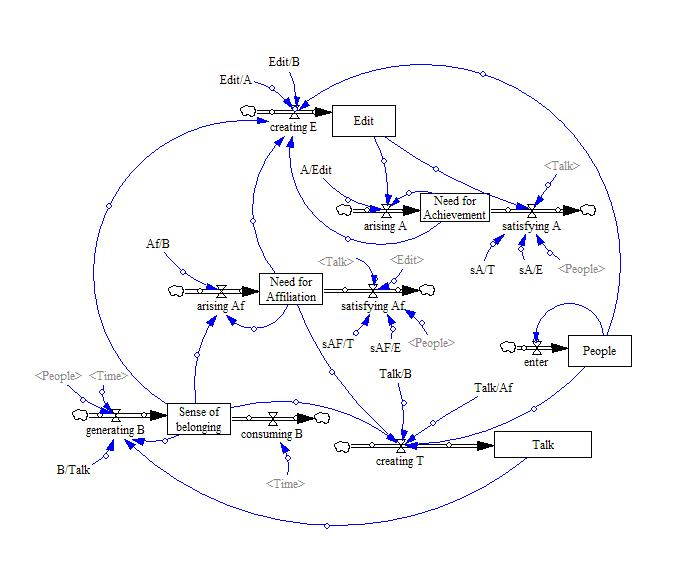
\includegraphics{06}}
  \caption{System dynamics model of motivation factors of Wikipedia community }
   \label{fig:sdmodel}
\end{figure}



\subsection{The comparison between system simulation results and the historical data of Wikipedia}
\label{sec:comp-betw-syst}

In order to prove the validity of the model, we present a comparison
between simulation results and the real historical data  which is
shown in fig. \ref{fig:comparison}. The historical data is gathered
from the statistics of Wikipedia, ranging from Jan, 2001 to May,
2006. The line of real data  is the increasing amount of edit activities
in Wikipedia community. If our model is effective enough, the
prediction of members behavior using this model, that is the amount of
edit, should close to the real data.  
The simulation results show that the system dynamics model is
approximately in accordance with the statistics in Wikipedia which
indicates the reasonability of using simulation results to explain the
motivation factors of Wikipedia members. We also see the big gap
between tow lines since July 2003 to April 2005. We believe the main
reason is  the sharply increasing edit amount and slowly
increasing Wikipedians amount during this period. According to Wikipedia
statistics\cite{wikistaten}, the increase of new Wikipedians and
contributors are relatively mild before 2005. Thus the group level of motivation
factors are not adaptive to the real edit behavior.   

\begin{figure}[htpb]
  \centering

  \scalebox{0.7}{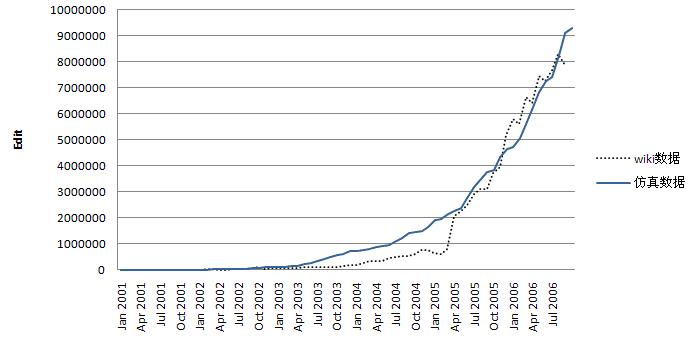
\includegraphics{07}}
  \caption{Comparison between system simulation results and the historical data }
\label{fig:comparison}
\end{figure}

\section{conclusion}
\label{sec:conclusion}

 In this study, we discussed motivation factors of knowledge
 collaboration in VCoP from individual level and group level. A system
 dynamics model is proposed to describe the feedback between motivation
 factors and how they affect the behavior of members in VCoP. We also
 use Wikipedia as a case to verify our model and the simulation shows
 our model is good for to reflect how motivation factors affect members' behavior.

The study also shows how a VCoP can  stimulate knowledge collaboration
from different aspects.
 First, on the individual level, the community should let others know
 about the individuals' contribution to make the individual feel
 respected. Meanwhile,  promote the contributors to higher level can
 effectively spurs their need for achievement. The friendly atmosphere
 is needed to stimulate their need for affiliation, which helps
 members to feel themselves as part of the community. As a result, the
 knowledge collaboration in VCoP is promoted. On the group level, the
 community operators should avail the members to discuss and interact
 with each other freely through IT infrastructures. The social
 interaction will promote the members' sense of belonging. Building
 the common impression and group consciousness, encouraging knowledge
 practice by improving their sense of identity are crucial to enhance
 collaboration . In addition, the community should be ready to
 discover the members' dissatisfaction with the community or new needs, and improve the community service to solve the conflicts between users or from system factors. The will of users to contribute to the community could be encouraged by improving their satisfaction with the community. 



\bibliographystyle{elsarticle-harv}
 % \bibliography{../../bibtex/elsevier,../../bibtex/emerald,../../bibtex/chinese,../../bibtex/jstor,../../bibtex/citeseer,../../bibtex/acm,../../bibtex/wiley,../../bibtex/book,../../bibtex/thesis,../../bibtex/ebsco,../../bibtex/old,../../bibtex/ieee,../../bibtex/internet,../../bibtex/ssrn,../../bibtex/apa,../../bibtex/blackwell,../../bibtex/sage,../../bibtex/springer,../../bibtex/MESharp,../../bibtex/taylor,../../bibtex/arXiv,../../bibtex/liebert}
\begin{thebibliography}{52}
\expandafter\ifx\csname natexlab\endcsname\relax\def\natexlab#1{#1}\fi
\expandafter\ifx\csname url\endcsname\relax
  \def\url#1{\texttt{#1}}\fi
\expandafter\ifx\csname urlprefix\endcsname\relax\def\urlprefix{URL }\fi

\bibitem[{Adler and Christopher(1998)}]{Christopher1998}
Adler, R., Christopher, A., 1998. Internet community primer: Overview and
  business opportunities.


\bibitem[{Amabile(1998)}]{amabile1998kc}
Amabile, T.~M., 1998. How to kill creativity. Harvard Business Review 76~(5),
  76-87.

\bibitem[{Bagozzi and Dholakia(2002)}]{richard_p._bagozzi_intentional_2002}
Bagozzi, R.~P., Dholakia, U.~M., 2002. Intentional social action in virtual
  communities. Journal of Interactive Marketing 16~(2), 2-21.


\bibitem[{Bartle(1996)}]{mud}
Bartle, R., 1996. Hearts, clubs, diamonds, spades: Players who suit muds.


\bibitem[{Beecham et~al.(2008)Beecham, Baddoo, Hall, Robinson, and
  Sharp}]{Beecham2008}
Beecham, S., Baddoo, N., Hall, T., Robinson, H., Sharp, H., Aug. 2008.
  Motivation in software engineering: A systematic literature review.
  Information and Software Technology 50~(9-10), 860-878.

\bibitem[{Bock et~al.(2005)Bock, Zmud, Kim, and Lee}]{1631336620050301}
Bock, G.-W., Zmud, R.~W., Kim, Y.-G., Lee, J.-N., 2005. Behavioral intention
  formation in knowledge sharing: Examining the roles of extrinsic motivators,
  social-psychological forces, and organizational climate. MIS Quarterly
  29~(1), 87-111.

\bibitem[{Bundura(1977)}]{bundura1977slt}
Bundura, A., 1977. Social Learning Theory. London: Prentice Hall.

\bibitem[{Clark et~al.(1994)Clark, Varadarajan, and Pride}]{clark1994emc}
Clark, T., Varadarajan, P., Pride, W., 1994. {Environmental management: The
  construct and research propositions}. Journal of Business Research 29~(1),
  23-38.

\bibitem[{Deci and Ryan(1985)}]{deci1985ima}
Deci, E., Ryan, R., 1985. Intrinsic Motivation and Self-Determination in Human
  Behavior. Springer.

\bibitem[{Deci and Ryan(2000)}]{deci2000agp}
Deci, E., Ryan, R., 2000. The" what" and" why" of goal pursuits: Human needs
  and the self-determination of behavior. Psychological Inquiry 11~(4),
  227-268.

\bibitem[{Deci et~al.(1999)Deci, Koestner, and Ryan}]{bul-125-6-62719991101}
Deci, E.~L., Koestner, R., Ryan, R.~M., 1999. A meta-analytic review of
  experiments examining the effects of extrinsic rewards on intrinsic
  motivation. Psychological Bulletin 125~(6), 627-668.

\bibitem[{Dholakia et~al.(2004)Dholakia, Bagozzi, and Pearo}]{dholakia2004241}
Dholakia, U.~M., Bagozzi, R.~P., Pearo, L.~K., 2004. A social influence model
  of consumer participation in network- and small-group-based virtual
  communities. International Journal of Research in Marketing 21~(3), 241-263.

\bibitem[{Diker(2004)}]{diker2004}
Diker, V., 2004. A dynamic feedback framework for studying growth policies in
  open online collaboration communitie. In: AMCIS 2004 Proceedings. p. 328.

\bibitem[{Eagly and Chaiken(1993)}]{eagly1993pa}
Eagly, A., Chaiken, S., 1993. {The psychology of attitudes}. Harcourt Brace
  Jovanovich College Publishers Fort Worth.

\bibitem[{Eisenberger and Armeli(1997)}]{eisenberger1997csr}
Eisenberger, R., Armeli, S., 1997. Can salient reward increase creative
  performance without reducing intrinsic creative interest? Journal of
  personality and social psychology 72~(3), 652-663.

\bibitem[{Eisenberger et~al.(1999{\natexlab{a}})Eisenberger, Pierce, and
  Cameron}]{eisenberger1999eri}
Eisenberger, R., Pierce, W., Cameron, J., 1999{\natexlab{a}}. Effects of reward
  on intrinsic motivation—negative, neutral, and positive: Comment on deci,
  koestner, and tyan. Psychological bulletin 125~(6), 677-691.

\bibitem[{Eisenberger et~al.(1999{\natexlab{b}})Eisenberger, Rhoades, and
  Carmeron}]{eisenberger1999dpp}
Eisenberger, R., Rhoades, L., Carmeron, J., 1999{\natexlab{b}}. Does pay for
  performance increase or decrease perceived self-determination and intrinsic
  motivation? Journal of personality and social psychology 77~(5), 1026-1040.

\bibitem[{Elliot(1999)}]{elliot1999aaa}
Elliot, A., 1999. {Approach and avoidance motivation and achievement goals}.
  Educational psychologist 34~(3), 169-189.

\bibitem[{Filkins et~al.(2000)Filkins, Allen, and
  Cordes}]{filkins2000predicting}
Filkins, R., Allen, J., Cordes, S., 2000. {Predicting community satisfaction
  among rural residents: An integrative model}. Rural Sociology 65~(1), 72-86.

\bibitem[{Flanagin and Metzger(2001)}]{flanagin2001internet}
Flanagin, A., Metzger, M., 2001. {Internet use in the contemporary media
  environment}. Human Communication Research 27~(1), 153-181.

\bibitem[{Gibbons(1998)}]{gibbons1998io}
Gibbons, R., 1998. Incentives in organizations. Journal of Economic
  Perspectives 12~(4), 115-132.

\bibitem[{Hagel~III and Armstrong(1997)}]{hagel1997net}
Hagel~III, J., Armstrong, A., 1997. {Net gain: expanding markets through
  virtual communities}. The McKinsey Quarterly~(1).

\bibitem[{Hsu et~al.(2007)Hsu, Ju, Yen, and Chang}]{Hsu2007}
Hsu, M.-H., Ju, T.~L., Yen, C.-H., Chang, C.-M., Feb. 2007. Knowledge sharing
  behavior in virtual communities: The relationship between trust,
  self-efficacy, and outcome expectations. International Journal of
  Human-Computer Studies 65~(2), 153-169.

\bibitem[{Kankanhalli et~al.(2005)Kankanhalli, Tan, and Wei}]{1631337020050301}
Kankanhalli, A., Tan, B. C.~Y., Wei, K.-K., 2005. Contributing knowledge to
  electronic knowledge repositories: An empirical investigation. MIS Quarterly
  29~(1), 113-143.

\bibitem[{Kasser(2002)}]{kasser2002hpm}
Kasser, T., 2002. The High Price of Materialism. Bradford Book.

\bibitem[{Kittur et~al.(2006)Kittur, Chi, Pendleton, Suh, and
  Mytkowicz}]{poweroffew}
Kittur, A., Chi, E., Pendleton, B., Suh, B., Mytkowicz, T., 2006. Power of the
  few vs. wisdom of the crowd: Wikipedia and the rise of the bourgeoisie.
  http://www.parc.com/research/publications/files/5904.pdf.

\bibitem[{Kozinets(1999)}]{Kozinets1999252}
Kozinets, R.~V., 1999. E-tribalized marketing?: the strategic implications of
  virtual communities of consumption. European Management Journal 17~(3), 252
  - 264.

\bibitem[{Kruglanski(1978)}]{Kruglanski1978}
Kruglanski, A., 1978. he Hidden Costs of Rewards, New Perspectives on the
  Psychology of Human Motivation. John Wiley, New York, Ch. Issues in cognitive
  social psychology,  19-30.

\bibitem[{Kuo and Young(2008)}]{Kuowiley2008}
Kuo, F.-Y., Young, M.-L., 2008. A study of the intention-action gap in
  knowledge sharing practices. Journal of the American Society for Information
  Science and Technology 59~(8), 1224-1237.


\bibitem[{Lazear(2000)}]{388530120001201}
Lazear, E.~P., 2000. Performance pay and productivity. American Economic Review
  90~(5), 1346 - 1361.

\bibitem[{Lerner and Tirole(2002)}]{josh_lerner_simple_2002}
Lerner, J., Tirole, J., 2002. Some simple economics of open source. Journal of
  Industrial Economics 50~(2), 197-234.


\bibitem[{Lin and Lee(2006)}]{lin2006determinants}
Lin, H., Lee, G., 2006. {Determinants of success for online communities: an
  empirical study}. Behaviour \& Information Technology 25~(6), 479-488.

\bibitem[{Lin(2007)}]{Hsiu-FenLin04012007}
Lin, H.-F., 2007. {Effects of extrinsic and intrinsic motivation on employee
  knowledge sharing intentions}. Journal of Information Science 33~(2),
  135-149.


\bibitem[{Lin(2008)}]{linhsiufen2008}
Lin, H.-F., 2008. Antecedents of virtual community satisfaction and loyalty: An
  empirical test of competing theories. CyberPsychology \& Behavior 11~(2),
  138-144, pMID: 18422404.



\bibitem[{Mao et~al.(2007)Mao, Vassileva, and Grassmann}]{4076734}
Mao, Y., Vassileva, J., Grassmann, W., Jan. 2007. A system dynamics approach to
  study virtual communities. In: System Sciences, 2007. HICSS 2007. 40th Annual
  Hawaii International Conference on. pp. 178a-178a.

\bibitem[{McClelland(1976)}]{mcclelland1976am}
McClelland, D., 1976. The Achievement Motive. Irvington Publishers: distributed
  by Halsted Press.

\bibitem[{McMillan and Chavis(1986)}]{mcmillan1986scd}
McMillan, D., Chavis, D., 1986. {Sense of community: A definition and theory}.
  Journal of Community Psychology 14~(1), 6-23.

\bibitem[{Mitzel et~al.(1982)Mitzel, Best, and
  Rabinowitz}]{mitzel1982encyclopedia}
Mitzel, H., Best, J., Rabinowitz, W., 1982. {Encyclopedia of educational
  research}. Simon \& Schuster Children's Publishing.

\bibitem[{Oliver(1980)}]{oliver1980cognitive}
Oliver, R., 1980. {A cognitive model of the antecedents and consequences of
  satisfaction decisions}. Journal of Marketing research, 460-469.

\bibitem[{Postmes et~al.(2000)Postmes, Spears, and
  Lea}]{t_postmes_formation_2000}
Postmes, T., Spears, R., Lea, M., 2000. The formation of group norms in
  computer-mediated communication. Human Communication Research 26~(3),
  341-371.


\bibitem[{Rheingold(2000)}]{rheingold2000vch}
Rheingold, H., 2000. {The virtual community: Homesteading on the electronic
  frontier}. MIT press.

\bibitem[{Ryan and Deci(2000)}]{Ryan200054}
Ryan, R.~M., Deci, E.~L., 2000. Intrinsic and extrinsic motivations: Classic
  definitions and new directions. Contemporary Educational Psychology 25~(1),
  54 - 67.

\bibitem[{Rønnow-Rasmussen(2002)}]{Roennow-Rasmussen2002}
Rønnow-Rasmussen, T., Mar. 2002. Instrumental values – strong and weak.
  Ethical Theory and Moral Practice 5~(1), 23-43.


\bibitem[{Schwartz(1990)}]{schwartz1993cad}
Schwartz, B., 1990. The creation and destruction of value. American
  Psychologist 45, 7-15.

\bibitem[{Shang et~al.(2005)Shang, Chen, and Shen}]{shang2005evi}
Shang, R., Chen, Y., Shen, L., 2005. {Extrinsic versus intrinsic motivations
  for consumers to shop on-line}. Information \& Management 42~(3), 401-413.

\bibitem[{Stavredes(2001)}]{stavredes2001system}
Stavredes, T., 2001. {A system dynamics evaluation model and methodology for
  instructional technology support}. Computers in Human Behavior 17~(4),
  409-419.

\bibitem[{Teo et~al.(1999)Teo, Lim, and Lai}]{teo1999iae}
Teo, T., Lim, V., Lai, R., 1999. {Intrinsic and extrinsic motivation in
  Internet usage}. Omega 27~(1), 25-37.

\bibitem[{Warren(1972)}]{warren1972ca}
Warren, R., 1972. {The community in America}. Rand McNally Chicago.

\bibitem[{Wikimedia(2009)}]{wikistaten}
Wikimedia, 2009. Wikipedia statistics.
  http://stats.wikimedia.org/EN/ChartsWikipediaEN.htm.

\bibitem[{Wilson et~al.(1981)Wilson, Hull, and Johnson}]{wilson1981aas}
Wilson, T., Hull, J., Johnson, J., 1981. Awareness and self-perception: Verbal
  reports on internal states. Journal of Personality and Social Psychology
  40~(1), 53-71.

\bibitem[{Wittmann and Hattrup(2004)}]{wittmann_relationship_2004}
Wittmann, W.~W., Hattrup, K., 2004. The relationship between performance in
  dynamic systems and intelligence. Systems Research and Behavioral Science
  21~(4), 393-409.


\bibitem[{Zhuge and Guo(2007)}]{Zhugea}
Zhuge, H., Guo, W., 2007. Virtual knowledge service market—for effective
  knowledge flow within knowledge grid. Journal of Systems and Software
  80~(11), 1833-1842.

\end{thebibliography}

\end{document}
